% Analisi dei requisiti

\chapter{Analisi dei requisiti}

% TODO: CTO e CEO in glossary?
% TODO: feature in glossary?
% TODO: beta tester in glossary?
PastBot nasce da un insieme di nuove tecnologie e dalla necessità di ampliare i
metodi a disposizione per l'acquisito di prodotti da PastBook.
La prima attività del progetto è stata dunque la consultazione del parere del
servizio Marketing e del CEO riguardo la creazione di un nuovo modo per
interagire con gli utenti. Dopo che la creazione di un bot per la piattaforma
Facebook è stata accolta, si è passati a valutare l'opinione di una parte
dell'utenza di PastBook. L'utenza ascoltata fa parte del gruppo di tester di
PastBook, che ha deciso di avere un accesso anticipato ai nuovi prodotti in
cambio di una loro valutazione. L'azienda si è rivolta a loro anche per valutare
l'interessamento nell'utilizzo di un futuro bot per Facebook, idea che è stata
accolta favorevolmente in buona parte.

Si è quindi passati all'interazione con il reparto di codifica, che ha dovuto
eseguire un'analisi dei requisiti per estrapolare i casi d'uso prima di poter
cominciare a progettare il prodotto.

\section{Requisiti di PastBot}

PastBot suddivide l'utenza in due categorie principali:
l'utenza non registrata, ovvero che non ha mai scritto al bot e
l'utenza registrata, cioè che ha almeno una volta scritto al bot.

\subsection{UC0: caso d'uso generale}
\label{uc:uc0}

\begin{figure}[H]
  \centering
  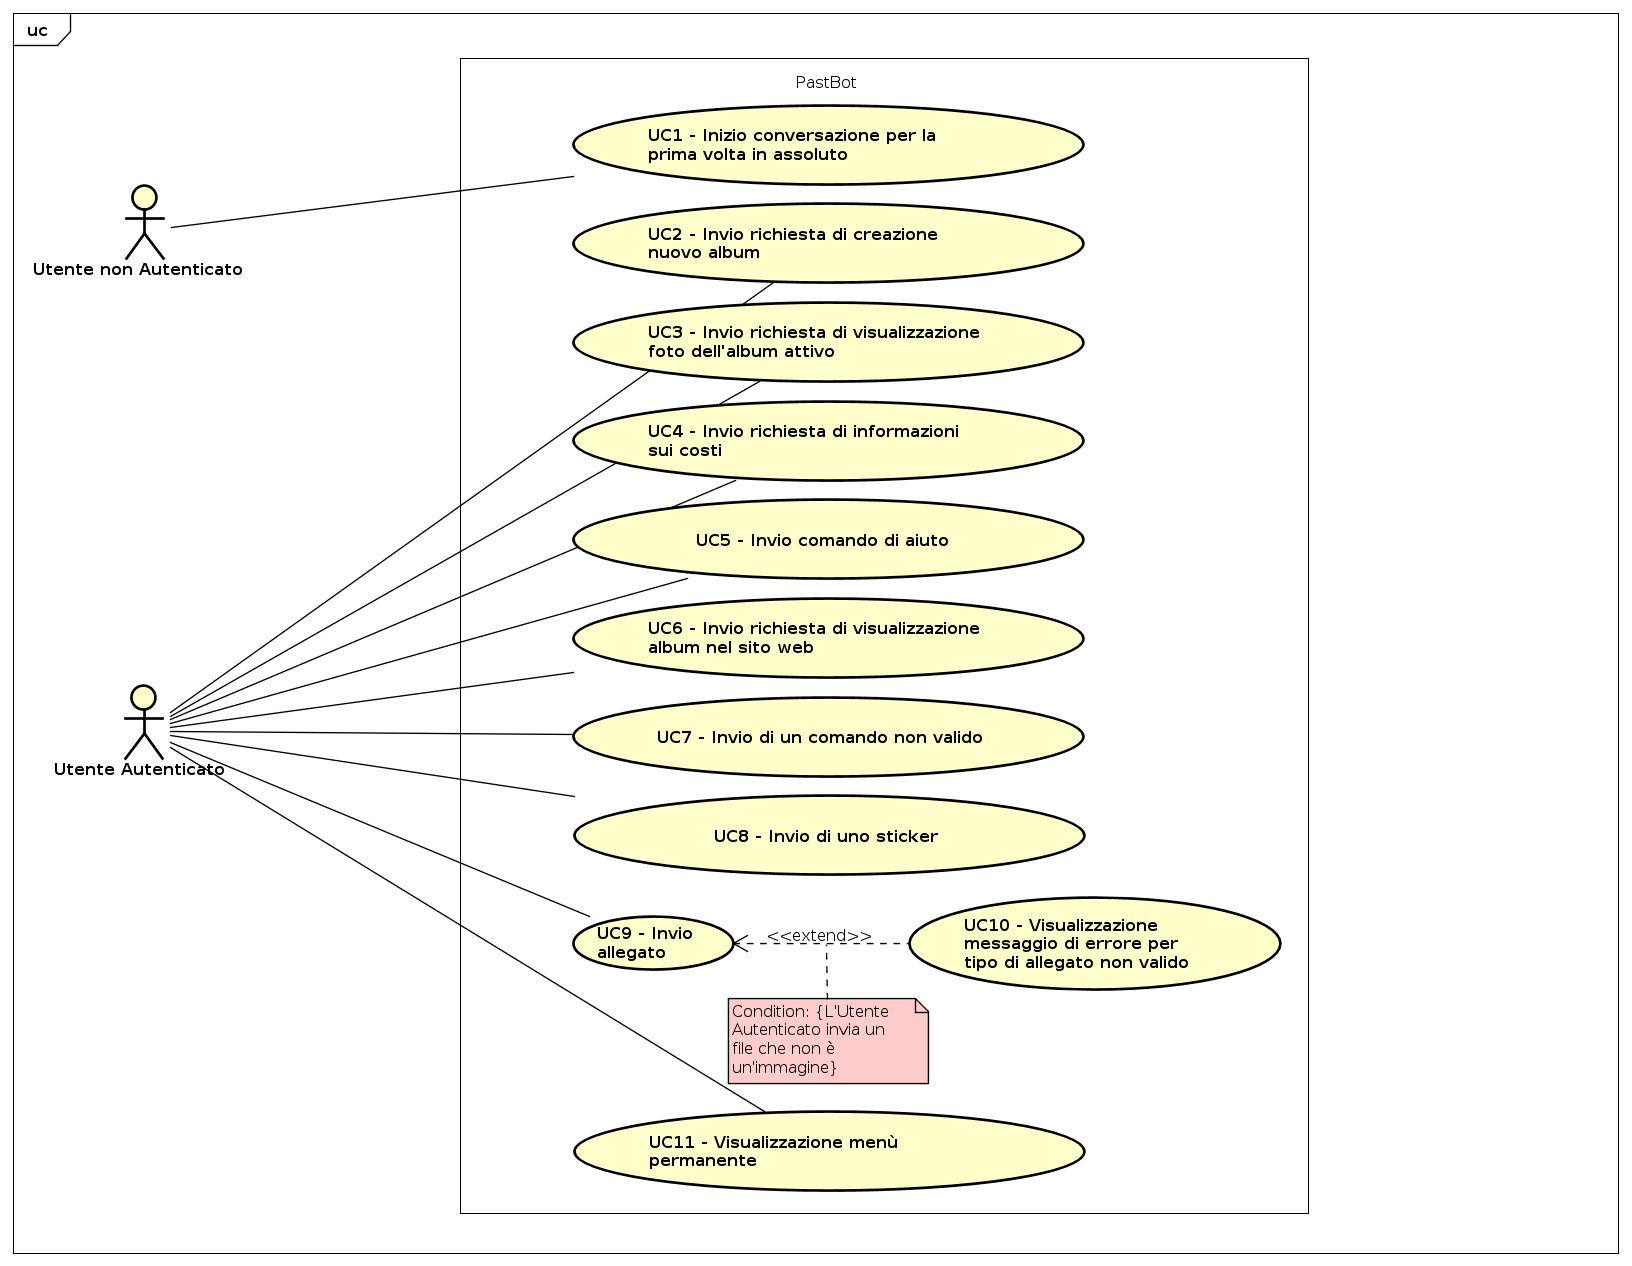
\includegraphics[scale=0.4]{useCase/UC0}
  \caption{UC0: caso d'uso generale}
\end{figure}

\begin{itemize}
  \item \textbf{Attori}: Utente Non Autenticato, Utente Autenticato;
  \item \textbf{Descrizione}: un utente inanzitutto deve iniziare la
conversazione con il bot. Dopo di che avrà a disposizione il sistema di
conversazione in cui poter mandare messaggi al bot;
  \item \textbf{Precondizione}: l'utente deve aver un account Messenger e deve
averci effettuato la connessione;
  \item \textbf{Postcondizione}: il sistema ha erogato le funzionalità
richieste dall'utente;
  \item \textbf{Flusso principale}:
  \begin{enumerate}
    \item L'Utente Non Autenticato può iniziare una conversazione per la prima
volta in assoluto
    \item L'Utente Autenticato può inviare una richiesta di creazione nuovo
album % FIXME: ref
    \item L'Utente Autenticato può inviare una richiesta visualizzazione album
esistente
    \item L'Utente Autenticato può inviare richiesta informazione sui costi
    \item L'Utente Autenticato può inviare comando di aiuto
    \item L'Utente Autenticato può inviare richiesta di visualizzazione
dell'album nel sito web
    \item L'Utente Autenticato può inviare un comando non valido
    \item L'Utente Autenticato può inviare uno \textit{sticker}
    \item L'Utente Autenticato può inviare un allegato % FIXME: ref
    \item L'Utente Autenticato può visualizzare il menù permanente.
  \end{enumerate}
  \item \textbf{Scenari alternativi}: nessuno.
\end{itemize}


% \newpage

\subsection{UC1: inizio conversazione per la prima volta in assoluto}
\label{uc:uc1}

\begin{itemize}
  \item \textbf{Attori}: Utente Non Autenticato;
  \item \textbf{Descrizione}: L'Utente Non Autenticato vuole scrivere al bot
per la prima volta in assoluto. Per fare questa azione dovrà premere il bottone
"Inizia" presente in Messenger.
  \item \textbf{Precondizione}: L'Utente Non Autenticato è iscritto alla
piattaforma di messaggistica Facebook Messenger
  \item \textbf{Postcondizione}: L'Utente Non Autenticato ha inviato con
successo il suo primo messaggio al bot
  \item \textbf{Flusso principale}:
  \begin{enumerate}
    \item L'Utente Non Autenticato clicca sul bottone apposito per iniziare la
conversazione
  \end{enumerate}
  \item \textbf{Scenari alternativi}: nessuno
\end{itemize}



%%% INIZIO SEZIONE USE CASE 2 %%%
\newpage

\subsection{UC2: invio richiesta di creazione di un nuovo album}
\label{uc:uc2}

\begin{figure}[H]
  \centering
  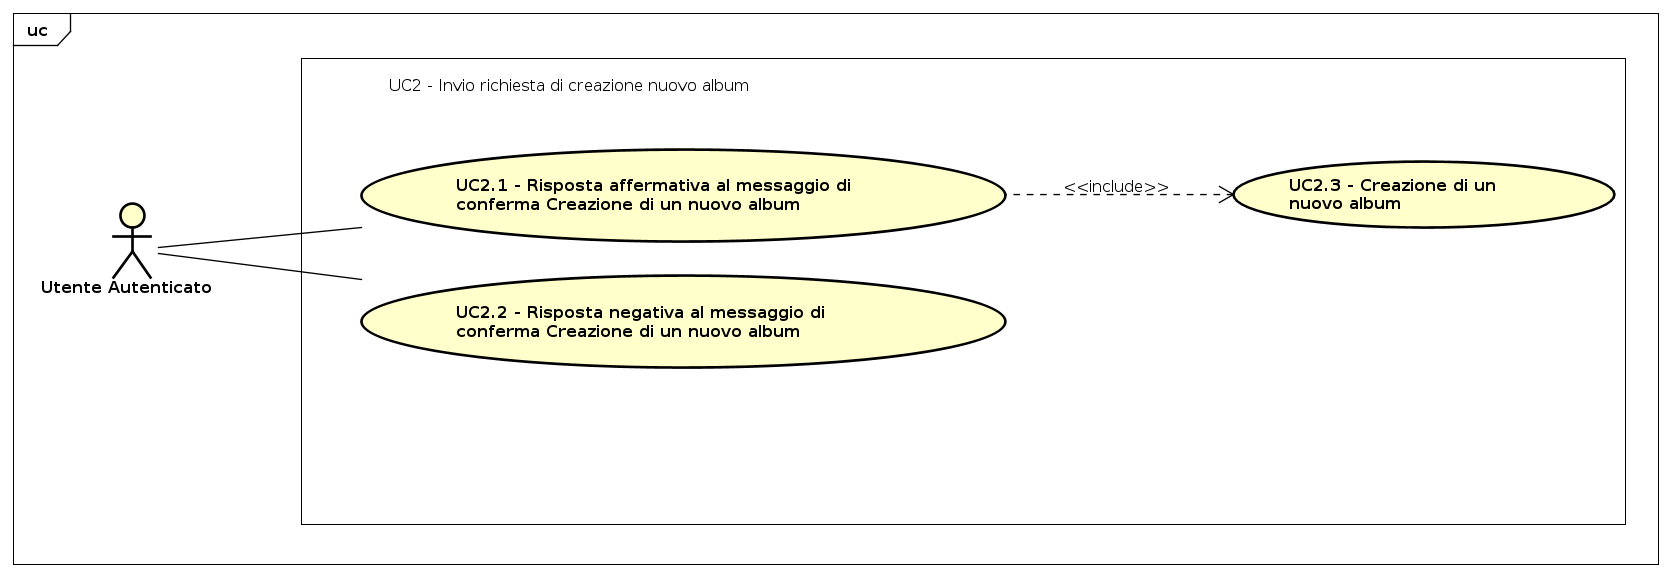
\includegraphics[scale=0.3]{useCase/UC2}
  \caption{UC2: invio richiesta di creazione di un nuovo album}
\end{figure}

\begin{itemize}
  \item \textbf{Attori}: Utente Autenticato;
  \item \textbf{Descrizione}: l'Utente Autenticato procede alla richiesta di
creazione di un nuovo album di foto. Gli verrà posta una domanda per avere
conferma della creazione, alla quale potrà rispondere in maniera affermativa o
negativa
  \item \textbf{Precondizione}: l'Utente Autenticato ha cominciato la
conversazione con il bot
  \item \textbf{Postcondizione}: l'Utente Autenticato ha gestito con successo
il proprio album
  \item \textbf{Flusso principale}:
  \begin{enumerate}
    \item L'Utente Autenticato conferma la creazione di un nuovo album
    \item L'Utente Autenticato non conferma la creazione di un nuovo album
  \end{enumerate}
  \item \textbf{Scenari alternativi}: nessuno.
\end{itemize}

%\newpage

\subsection{UC2.1: risposta affermativa al messaggio di conferma Creazione
nuovo album}
\label{uc:uc2.1}

\begin{itemize}
  \item \textbf{Attori}: Utente Autenticato;
  \item \textbf{Descrizione}: L'Utente Autenticato conferma la decisione di
voler creare un nuovo album
  \item \textbf{Precondizione}: L'Utente Autenticato ha richiesto la creazione
di un nuovo album
  \item \textbf{Postcondizione}: L'Utente Autenticato ha confermato con
successo la volontà di creare un nuovo album
  \item \textbf{Flusso principale}:
  \begin{enumerate}
    \item L'Utente Autenticato conferma positivamente la creazione di un nuovo
album
  \end{enumerate}
  \item \textbf{Scenari alternativi}: nessuno
\end{itemize}


%\newpage

\subsection{UC2.2: risposta negativa al messaggio di conferma Creazione nuovo
album}
\label{uc:uc2.2}

\begin{itemize}
  \item \textbf{Attori}: Utente Autenticato;
  \item \textbf{Descrizione}: L'Utente Autenticato decide di non voler più
creare un nuovo album
  \item \textbf{Precondizione}: L'Utente Autenticato ha richiesto la creazione
di un nuovo album
  \item \textbf{Postcondizione}: L'Utente Autenticato ha confermato con
successo la volontà di non procedere alla creazione di un nuovo album
  \item \textbf{Flusso principale}:
  \begin{enumerate}
    \item L'Utente Autenticato conferma negativamente la creazione di un nuovo
album
  \end{enumerate}
  \item \textbf{Scenari alternativi}: nessuno
\end{itemize}


%\newpage

\subsection{UC2.3: creazione di un nuovo album}
\label{uc:uc2.3}

\begin{itemize}
  \item \textbf{Attori}: Utente Autenticato;
  \item \textbf{Descrizione}: Si ottiene un nuovo album vuoto in cui sarà
possibile inserire nuove foto
  \item \textbf{Precondizione}: L'Utente Autenticato ha confermato
positivamente la volontà di creare un nuovo album
  \item \textbf{Postcondizione}: L'Utente Autenticato dispone di un nuovo album
  \item \textbf{Flusso principale}:
  \begin{enumerate}
    \item L'Utente Autenticato ha confermato positivamente la creazione di un
nuovo album
  \end{enumerate}
  \item \textbf{Scenari alternativi}: nessuno
\end{itemize}


%%% FINE SEZIONE USE CASE 2 %%%

%%% INIZIO SEZIONE USE CASE 3 %%%
\newpage

\subsection{UC3: invio richiesta di visualizzazione foto dell'album attivo}
\label{uc:uc3}

% FIXME: manca scenario alternativo in UC0.png in cui se viene richiesta una
%lista di un album senza nulla viene segnalato un messaggio di errore.

\begin{figure}[H]
  \centering
  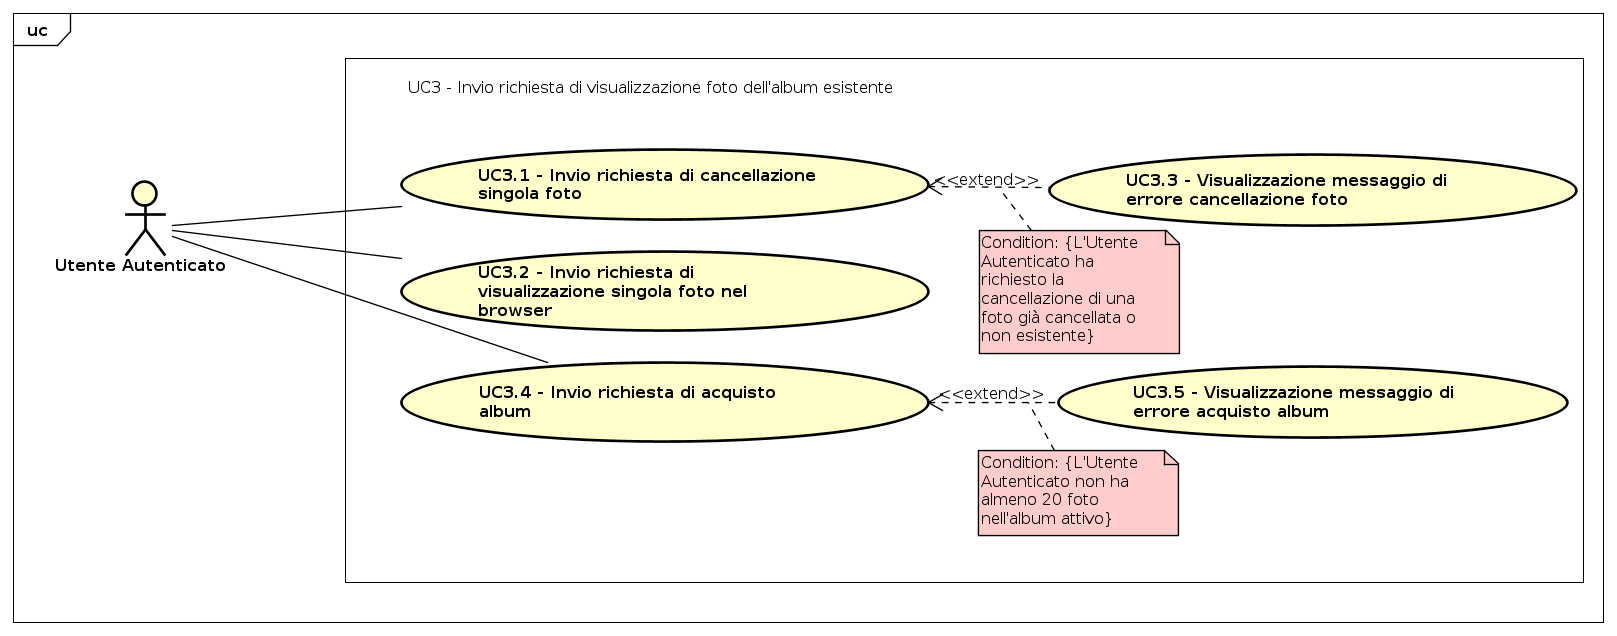
\includegraphics[scale=0.35]{useCase/UC3}
  \caption{UC3: invio richiesta di visualizzazione foto dell'album attivo}
\end{figure}

\begin{itemize}
  \item \textbf{Attori}: Utente Autenticato;
  \item \textbf{Descrizione}: l'Utente può richiedere la visualizzazione della
lista delle foto attualmente caricate, su cui può decidere di cancellarne
alcune, di visualizzarle senza perdita di risoluzione di di acquistarle in un
album.
  \item \textbf{Precondizione}: l'Utente Autenticato ha cominciato la
conversazione con il bot
  \item \textbf{Postcondizione}: l'Utente Autenticato ha visualizzato con
successo la lista delle foto presenti nel proprio album
  \item \textbf{Flusso principale}:
  \begin{enumerate}
    \item L'Utente Autenticato cancella una singola foto dall'album
    \item L'Utente Autenticato visualizza una singola foto dell'album alla
massima risoluzione disponibile
    \item L'Utente Autenticato richiede l'acquisto dell'album
  \end{enumerate}
  \item \textbf{Scenari alternativi}: nessuno
\end{itemize}


%\newpage

\subsection{UC3.1: cancellazione singola foto}
\label{uc:uc3.1}


\begin{itemize}
  \item \textbf{Attori}: Utente Autenticato;
  \item \textbf{Descrizione}: L'Utente Autenticato richiede la cancellazione di
una foto dall'album
  \item \textbf{Precondizione}: L'Utente Autenticato ha la lista delle foto
presenti nell'album
  \item \textbf{Postcondizione}: L'Utente Autenticato ha rimosso con successo
una foto dall'album
  \item \textbf{Flusso principale}:
  \begin{enumerate}
    \item L'Utente Autenticato invia la richiesta per rimuovere una foto
dall'album
  \end{enumerate}
  \item \textbf{Scenari alternativi}:
  \begin{enumerate}
    \item L'Utente Autenticato riceve un messaggio di errore nella
cancellazione della foto \ref{uc:uc3.3}
  \end{enumerate}
\end{itemize}


%\newpage

\subsection{UC3.2: visualizzazione singola foto nel browser}
\label{uc:uc3.2}

\begin{itemize}
  \item \textbf{Attori}: Utente Autenticato;
  \item \textbf{Descrizione}: L'Utente Autenticato vuole visualizzare in maniera
dettagliata e con la massima qualità disponibile una foto presente nell'album
  \item \textbf{Precondizione}: L'Utente Autenticato ha la lista delle foto
presenti nell'album
  \item \textbf{Postcondizione}: L'Utente Autenticato ha visualizzato con
successo una foto dall'album
  \item \textbf{Flusso principale}:
  \begin{enumerate}
    \item L'Utente Autenticato visualizza la foto dall'album
  \end{enumerate}
  \item \textbf{Scenari alternativi}: nessuno
\end{itemize}


%\newpage

\subsection{UC3.3: visualizzazione messaggio di errore cancellazione foto}
\label{uc:uc3.3}

\begin{itemize}
  \item \textbf{Attori}: Utente Autenticato;
  \item \textbf{Descrizione}: Questo caso si verifica quando l'Utente
Autenticato ordina la cancellazione di una foto già cancellata o ordina la
cancellazione di una foto di un album non più esistente.
  \item \textbf{Precondizione}: L'Utente Autenticato ha ordinato la
cancellazione di una foto non esistente o già cancellata
  \item \textbf{Postcondizione}: L'Utente Autenticato ha visualizzato il
messaggio di errore
  \item \textbf{Flusso principale}:
  \begin{enumerate}
    \item L'Utente Autenticato riceve un messaggio di errore nel tentativo di
cancellare una specifica foto
  \end{enumerate}
  \item \textbf{Scenari alternativi}: nessuno
\end{itemize}


%\newpage

\subsection{UC3.4: acquisto album}
\label{uc:uc3.4}

\begin{itemize}
  \item \textbf{Attori}: Utente Autenticato;
  \item \textbf{Descrizione}: L'Utente Autenticato è soddisfatto dell'album
creato e vuole procederne all'acquisto.
  \item \textbf{Precondizione}: L'Utente Autenticato ha la lista delle foto
presenti nell'album e in quell'album ci sono almeno 20 foto
  \item \textbf{Postcondizione}: L'Utente Autenticato ha acquistato con
successo l'album
  \item \textbf{Flusso principale}:
  \begin{enumerate}
    \item L'Utente Autenticato acquista l'album
  \end{enumerate}
  \item \textbf{Scenari alternativi}:
  \begin{enumerate}
    \item L'Utente Autenticato ottiene un messaggio di errore di acquisto album
\ref{uc:uc3.5}
  \end{enumerate}
\end{itemize}

%\newpage

\subsection{UC3.5: visualizzazione messaggio di errore acquisto album}
\label{uc:uc3.5}

\begin{itemize}
  \item \textbf{Attori}: Utente Autenticato;
  \item \textbf{Descrizione}: Questo errore avviene quando l'Utente Autenticato
tenta di acquistare un album con meno di venti fotografie
  \item \textbf{Precondizione}: L'Utente Autenticato ha richiesto l'acquisto
dell'album
  \item \textbf{Postcondizione}: L'Utente Autenticato ha visualizzato il
messaggio di errore
  \item \textbf{Flusso principale}:
  \begin{enumerate}
    \item L'Utente Autenticato riceve un messaggio di errore relativo
all'impossibilità di effettuare l'acquisto per mancanza di foto
  \end{enumerate}
  \item \textbf{Scenari alternativi}: nessuno
\end{itemize}


%%% FINE SEZIONE USE CASE 3 %%%


%\newpage

\subsection{UC4: invio richiesta di informazioni sui costi}
\label{uc:uc4}

\begin{itemize}
  \item \textbf{Attori}: Utente Autenticato;
  \item \textbf{Descrizione}: permette all'Utente Autenticato di avere
informazioni riguardo ai costi degli album e ai relativi costi di spedizione
  \item \textbf{Precondizione}: L'Utente Autenticato ha cominciato la
conversazione con il bot
  \item \textbf{Postcondizione}: L'Utente Autenticato ha visualizzato con
successo le informazioni sui costi
  \item \textbf{Flusso principale}:
  \begin{enumerate}
    \item L'Utente Autenticato richiede le informazioni relative ai costi
  \end{enumerate}
  \item \textbf{Scenari alternativi}: nessuno
\end{itemize}


%\newpage

\subsection{UC5: invio comando di aiuto}
\label{uc:uc5}

\begin{itemize}
  \item \textbf{Attori}: Utente Autenticato;
  \item \textbf{Descrizione}: in caso l'Utente Autenticato si trovi in una
situazione di difficoltà e non sappia quale operazione intraprendere, ha la
possibilità di chiedere aiuto per ricevedere delle istruzioni su come
utilizzare PastBot
  \item \textbf{Precondizione}: L'Utente Autenticato ha cominciato la
conversazione con il bot
  \item \textbf{Postcondizione}: L'Utente Autenticato ha visualizzato con
successo le istruzioni sull'utilizzo di PastBot
  \item \textbf{Flusso principale}:
  \begin{enumerate}
    \item L'Utente Autenticato richiede le informazioni sull'utilizzo di
PastBot
  \end{enumerate}
  \item \textbf{Scenari alternativi}: nessuno
\end{itemize}


%\newpage

\subsection{UC6: invio richiesta di visualizzazione album nel sito web}
\label{uc:uc6}

\begin{itemize}
  \item \textbf{Attori}: Utente Autenticato;
  \item \textbf{Descrizione}: è possibile visualizzare l'album nel sito web
dell'azienda
  \item \textbf{Precondizione}: l'Utente Autenticato ha cominciato la
conversazione con il bot
  \item \textbf{Postcondizione}: l'Utente Autenticato viene reindirizzato al
sito della compagnia con successo
  \item \textbf{Flusso principale}:
  \begin{enumerate}
    \item l'Utente Autenticato invia la richiesta di visualizzare l'album nel
sito della compagnia
  \end{enumerate}
  \item \textbf{Scenari alternativi}: nessuno
\end{itemize}

%\newpage

\subsection{UC7: invio di un comando non valido}
\label{uc:uc7}

\begin{itemize}
  \item \textbf{Attori}: Utente Autenticato;
  \item \textbf{Descrizione}: è possibile che venga inviato un comando non
interpretabile da parte di PastBot. Questo farà mandare a PastBot un messaggio
con le istruzioni e il suo utilizzo
  \item \textbf{Precondizione}: l'Utente Autenticato ha cominciato la
conversazione con il bot
  \item \textbf{Postcondizione}: l'Utente Autenticato riceve con successo un
messaggio di aiuto
  \item \textbf{Flusso principale}:
  \begin{enumerate}
    \item l'Utente Autenticato invia un comando non valido per PastBot
  \end{enumerate}
  \item \textbf{Scenari alternativi}: nessuno
\end{itemize}


%\newpage

\subsection{UC8: invio di uno sticker}
\label{uc:uc8}

\begin{itemize}
  \item \textbf{Attori}: Utente Autenticato;
  \item \textbf{Descrizione}: è possibile da parte degli utenti che utilizzano
la piattaforma di chat Messenger inviare anche degli \textit{stickers} a PastBot
  \item \textbf{Precondizione}: l'Utente Autenticato ha cominciato la
conversazione con il bot
  \item \textbf{Postcondizione}: l'Utente Autenticato visualizza con successo
la risposta di PastBot
  \item \textbf{Flusso principale}:
  \begin{enumerate}
    \item l'Utente Autenticato invia uno \textit{sticker}
  \end{enumerate}
  \item \textbf{Scenari alternativi}: nessuno
\end{itemize}


%\newpage

\subsection{UC9: invio allegato}
\label{uc:uc9}

\begin{itemize}
  \item \textbf{Attori}: Utente Autenticato;
  \item \textbf{Descrizione}: Si ha la possibilità di inviare degli allegati a
PastBot, per esempio per poter popolare il proprio album con delle immagini.
  \item \textbf{Precondizione}: l'Utente Autenticato ha cominciato la
conversazione con il bot
  \item \textbf{Postcondizione}: l'Utente Autenticato visualizza un messaggio
di successo di salvataggio dell'allegato
  \item \textbf{Flusso principale}:
  \begin{enumerate}
    \item l'Utente Autenticato invia un allegato a PastBot
  \end{enumerate}
  \item \textbf{Scenari alternativi}:
  \begin{enumerate}
    \item visualizzazione messaggio di errore per tipo di allegato non valido
    %ref da inserire per UC10
  \end{enumerate}
\end{itemize}


%\newpage
%
%\subsection{UC10: invio richiesta di creazione di un nuovo album}
%\label{uc:uc10}

%\begin{itemize}
%  \item \textbf{Attori}: Utente Non Autenticato, Utente Autenticato;
%  \item \textbf{Descrizione}:
%  \item \textbf{Precondizione}:
%  \item \textbf{Postcondizione}:
%  \item \textbf{Flusso principale}:
%  \begin{enumerate}
%    \item
%  \end{enumerate}
%  \item \textbf{Scenari alternativi}:
%\end{itemize}


\newpage

\subsection{UC11: visualizzazione menù permanente}
\label{uc:uc11}

\begin{figure}[H]
  \centering
  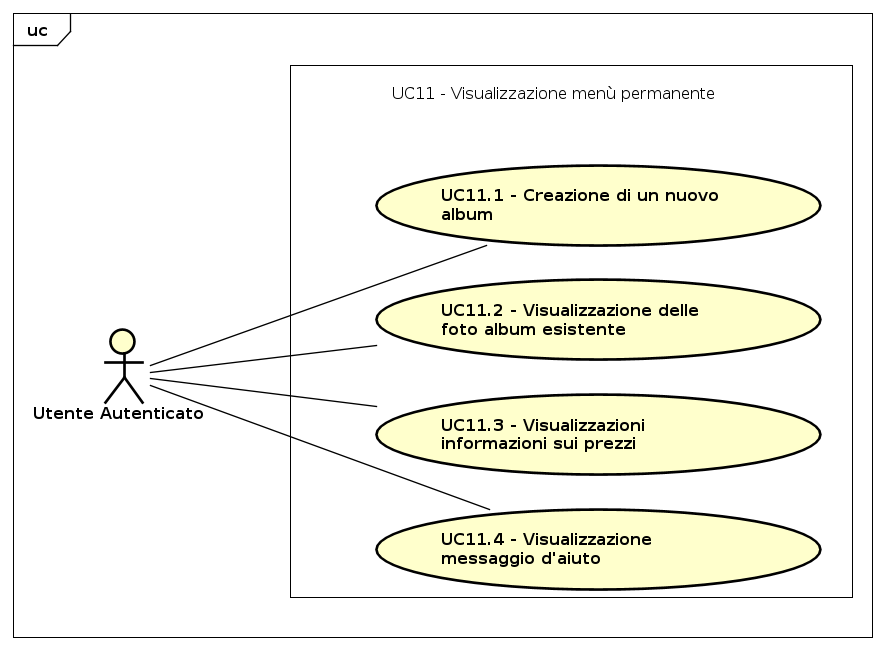
\includegraphics[scale=0.5]{useCase/UC11}
  \caption{UC11: visualizzazione menù permanente}
\end{figure}

\begin{itemize}
  \item \textbf{Attori}: Utente Autenticato;
  \item \textbf{Descrizione}: l'Utente Autenticato ha accesso al menù
permanente con il quale può inviare comandi al bot senza doverli inserire
tramite la tastiera.
  \item \textbf{Precondizione}: l'Utente Autenticato ha cominciato la
conversazione con il bot
  \item \textbf{Postcondizione}: l'Utente Autenticato esegue le operazioni
desiderate con successo
  \item \textbf{Flusso principale}:
  \begin{enumerate}
    \item L'Utente Autenticato effettua la richiesta di creazione di un nuovo
album
    \item L'Utente Autenticato richiede la visualizzazione delle foto esistenti
nell'ultimo album creato
    \item L'Utente Autenticato richiede le informazioni sui prezzi
    \item L'Utente Autenticato richiede la visualizzazione del messaggio di
aiuto
  \end{enumerate}
  \item \textbf{Scenari alternativi}: nessuno
\end{itemize}


%\newpage

\subsection{UC11.1: creazione di un nuovo album}
\label{uc:uc11.1}

\begin{itemize}
  \item \textbf{Attori}: Utente Autenticato;
  \item \textbf{Descrizione}: Ciò permette all'Utente Autenticato di creare un
nuovo album semplicemente cliccando un bottone.
  \item \textbf{Precondizione}: L'Utente Autenticato ha aperto il menù
permanente
  \item \textbf{Postcondizione}: L'Utente Autenticato ha inviato la richiesta
di creazione di un nuovo album con successo
  \item \textbf{Flusso principale}:
  \begin{enumerate}
    \item L'Utente Autenticato richiede la creazione di un nuovo album
  \end{enumerate}
  \item \textbf{Scenari alternativi}: nessuno
\end{itemize}


%\newpage

\subsection{UC11.2: visualizzazione delle foto dell'album esistente}
\label{uc:uc11.2}

\begin{itemize}
  \item \textbf{Attori}: Utente Autenticato;
  \item \textbf{Descrizione}: Tramite questa funzionalità sarà possibile per
l'Utente Autenticato visualizzare le foto che ha presenti nell'album in maneira
semplice
  \item \textbf{Precondizione}: L'Utente Autenticato ha aperto il menù
permanente
  \item \textbf{Postcondizione}: L'Utente Autenticato ha inviato la richiesta
di visualizzazione delle foto di un album esistente con successo
  \item \textbf{Flusso principale}:
  \begin{enumerate}
    \item L'Utente Autenticato richiede la visualizzazione delle foto di un
album
  \end{enumerate}
  \item \textbf{Scenari alternativi}: % FIXME: manca caso d'uso in cui l'album
%è vuoto
\end{itemize}

% TODO: descrizione di tutti gli altri casi d'uso senza l'immagine!



% TEMPLATE USECASE
%\newpage
%
%\subsection{UC2: invio richiesta di creazione di un nuovo album}
%\label{uc:uc2}

%\begin{figure}[H]
%  \centering
%  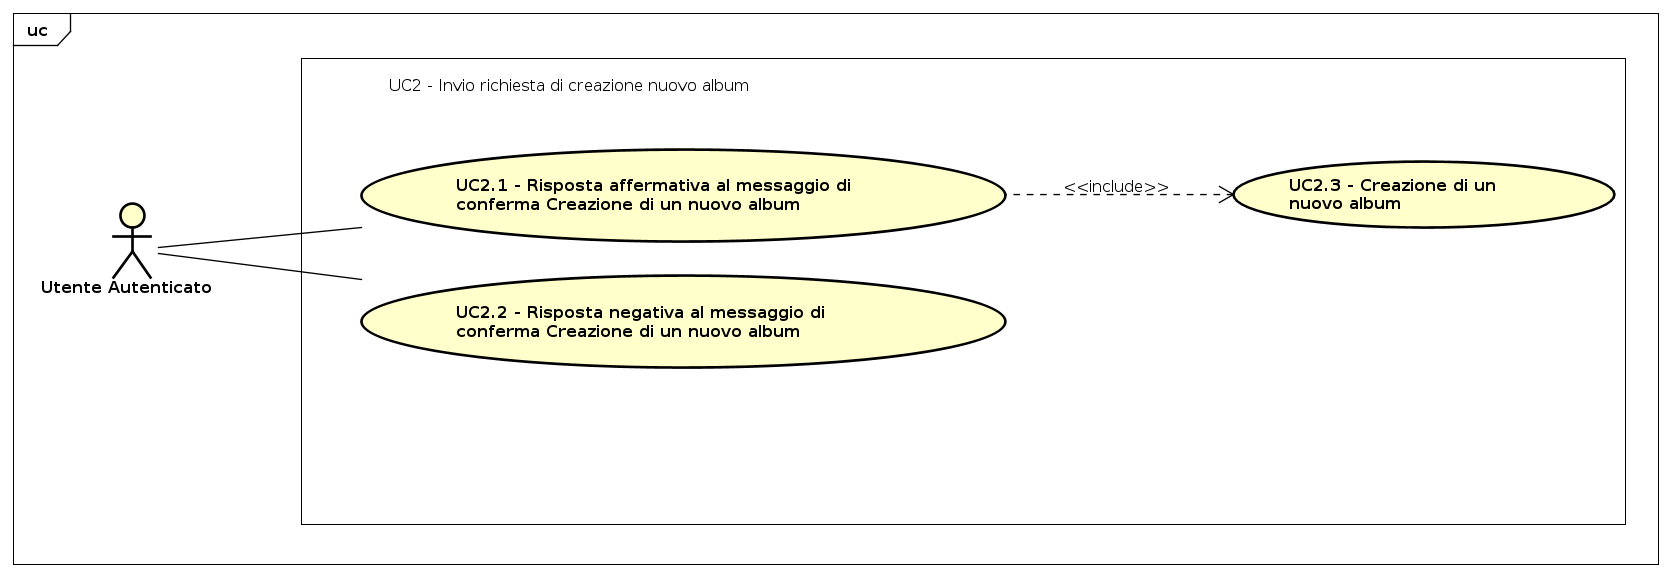
\includegraphics[scale=0.5]{useCase/UC2}
%  \caption{UC2: invio richiesta di creazione di un nuovo album}
%\end{figure}
%
%\begin{itemize}
%  \item \textbf{Attori}: Utente Non Autenticato, Utente Autenticato;
%  \item \textbf{Descrizione}:
%  \item \textbf{Precondizione}:
%  \item \textbf{Postcondizione}:
%  \item \textbf{Flusso principale}:
%  \begin{enumerate}
%    \item
%  \end{enumerate}
%  \item \textbf{Scenari alternativi}:
%\end{itemize}
